\section{Machine Learning for the Cluster Reconstruction in the CALIFA Calorimeter at R$^3$B}

This study on improving cluster reconstruction in CALIFA using machine learning techniques was initiated in the context of data analysis for the S455 experiment, \textit{``Fission via Quasi-Free Scattering Reaction: $^{238}$U$(p,2p)X$''} (see Section~\ref{sec:fission_qfs}). The R$^3$B setup is designed to enable complete kinematic reconstruction of nuclear reactions. In the case of quasi-free scattering (QFS)-induced fission, as studied in S455, this implies that, in addition to reconstructing both heavy and light fission fragments via the dedicated SOFIA setup and detecting neutrons with the large-area NeuLAND detector, it is also possible to identify the two correlated protons from the QFS process. Furthermore, CALIFA can be used to detect the gamma rays emitted during the de-excitation of the fission fragments.\newline
This capability enables precise measurements of the evolution of fission probabilities as a function of excitation energy ($E^*$), as well as the determination of fission barrier heights. These observables are particularly relevant for the study of short-lived, exotic nuclei, for which experimental data are scarce.\newline
The S455 experiment, performed with a stable $^{238}$U beam, served as a pilot study and proof of principle for this novel experimental approach. A key objective was to tag specific isotopes and analyze the associated gamma-ray spectra measured with CALIFA. For light actinides such as uranium, fission is predominantly characterized by asymmetric mass splitting, a consequence of shell effects~\cite{sartori2013nuclear}, which results in a strong population of tin isotopes ($Z = 50$). These isotopes are of particular interest for gamma spectroscopy due to their well-known structure and high-lying excited states. Accordingly, a selection on $Z = 50$ fragments was applied, accounting for sufficient production cross-section with the presence of prominent gamma transitions. Notably, $^{132}$Sn exhibits a $2^+$ state at 4.041~MeV~\cite{schopper2013excited}, well above CALIFA's gamma detection threshold of approximately 200~keV, and should therefore be clearly identifiable.\newline
Initial attempts to reconstruct gamma spectra via Doppler correction for $Z = 50$ fragments, however, yielded unsatisfactory results. The resulting spectra displayed broad distributions with no discernible peaks. Several factors contribute to the difficulty of accurate gamma energy reconstruction in this context, amongst others:\newline
\textbf{High Background from Delta Electrons:} In heavy-ion fission experiments, numerous delta electrons are generated due to interactions between the beam particles and atomic electrons in the target and surrounding materials. These electrons create a significant number of spurious hits in CALIFA, which interfere with gamma cluster reconstruction and degrade the energy resolution.\newline
\textbf{High-Energy Gamma Emission:} The de-excitation gamma rays from fission fragments often possess very high energies, especially in the laboratory frame at beam energies of 540~AMeV, where $E_{\text{lab}} > 10$~MeV. This is well above the pair production threshold (1.022~MeV), making pair production the dominant interaction mechanism. Consequently, gamma-ray interactions lead to more widely distributed and sparse detector hits, further complicating the clustering and energy reconstruction process.\newline
These challenges, along with the difficulty in extracting meaningful gamma spectra, motivated a collaboration with the \textit{Origins Data Science Lab (ODSL)} to explore advanced machine learning techniques for improving gamma cluster reconstruction in CALIFA.\newline
This section is structured as follows:\newline
First, the specific challenges associated with clustering in relativistic gamma spectroscopy are discussed. Subsequently, the standard clustering model implemented in the R3BRoot framework--used for both online and offline analysis of experimental data within the R3B setup--is reviewed.\newline
Next, the simulation framework and settings used for evaluating and comparing the performance of different clustering algorithms are introduced, along with the performance metrics used.\newline
The agglomerative clustering model, an unsupervised learning approach that incorporates hit time information in CALIFA, is then presented.\newline
This is followed by a description of the Edge Detection Neural Network, developed to improve clustering performance, particularly in the presence of complex hit patterns at the edges of clusters.\newline
Finally, the performance of the proposed models is assessed, including a comparison with selected hand-labeled event examples, where the neural network-based model demonstrates superior results.

\subsection{Gamma Spectroscopy with the Standard R3B Clustering Algorithm}
\subsubsection{Challenges in Relativistic Gamma Spectroscopy}
While the detection of light charged particles such as protons typically yields well-localized energy deposits in segmented detector arrays, the detection of gamma rays which emerge from the reaction vertex presents significant challenges. These difficulties primarily arise from the inherently sparse and spatially distributed energy deposits resulting from the interaction mechanisms of photons with the scintillator material (see Fig. \ref{fig:csi}) \cite{kolanoski2016teilchendetektoren}.\newline
\begin{figure}[!htb]
        \centering
        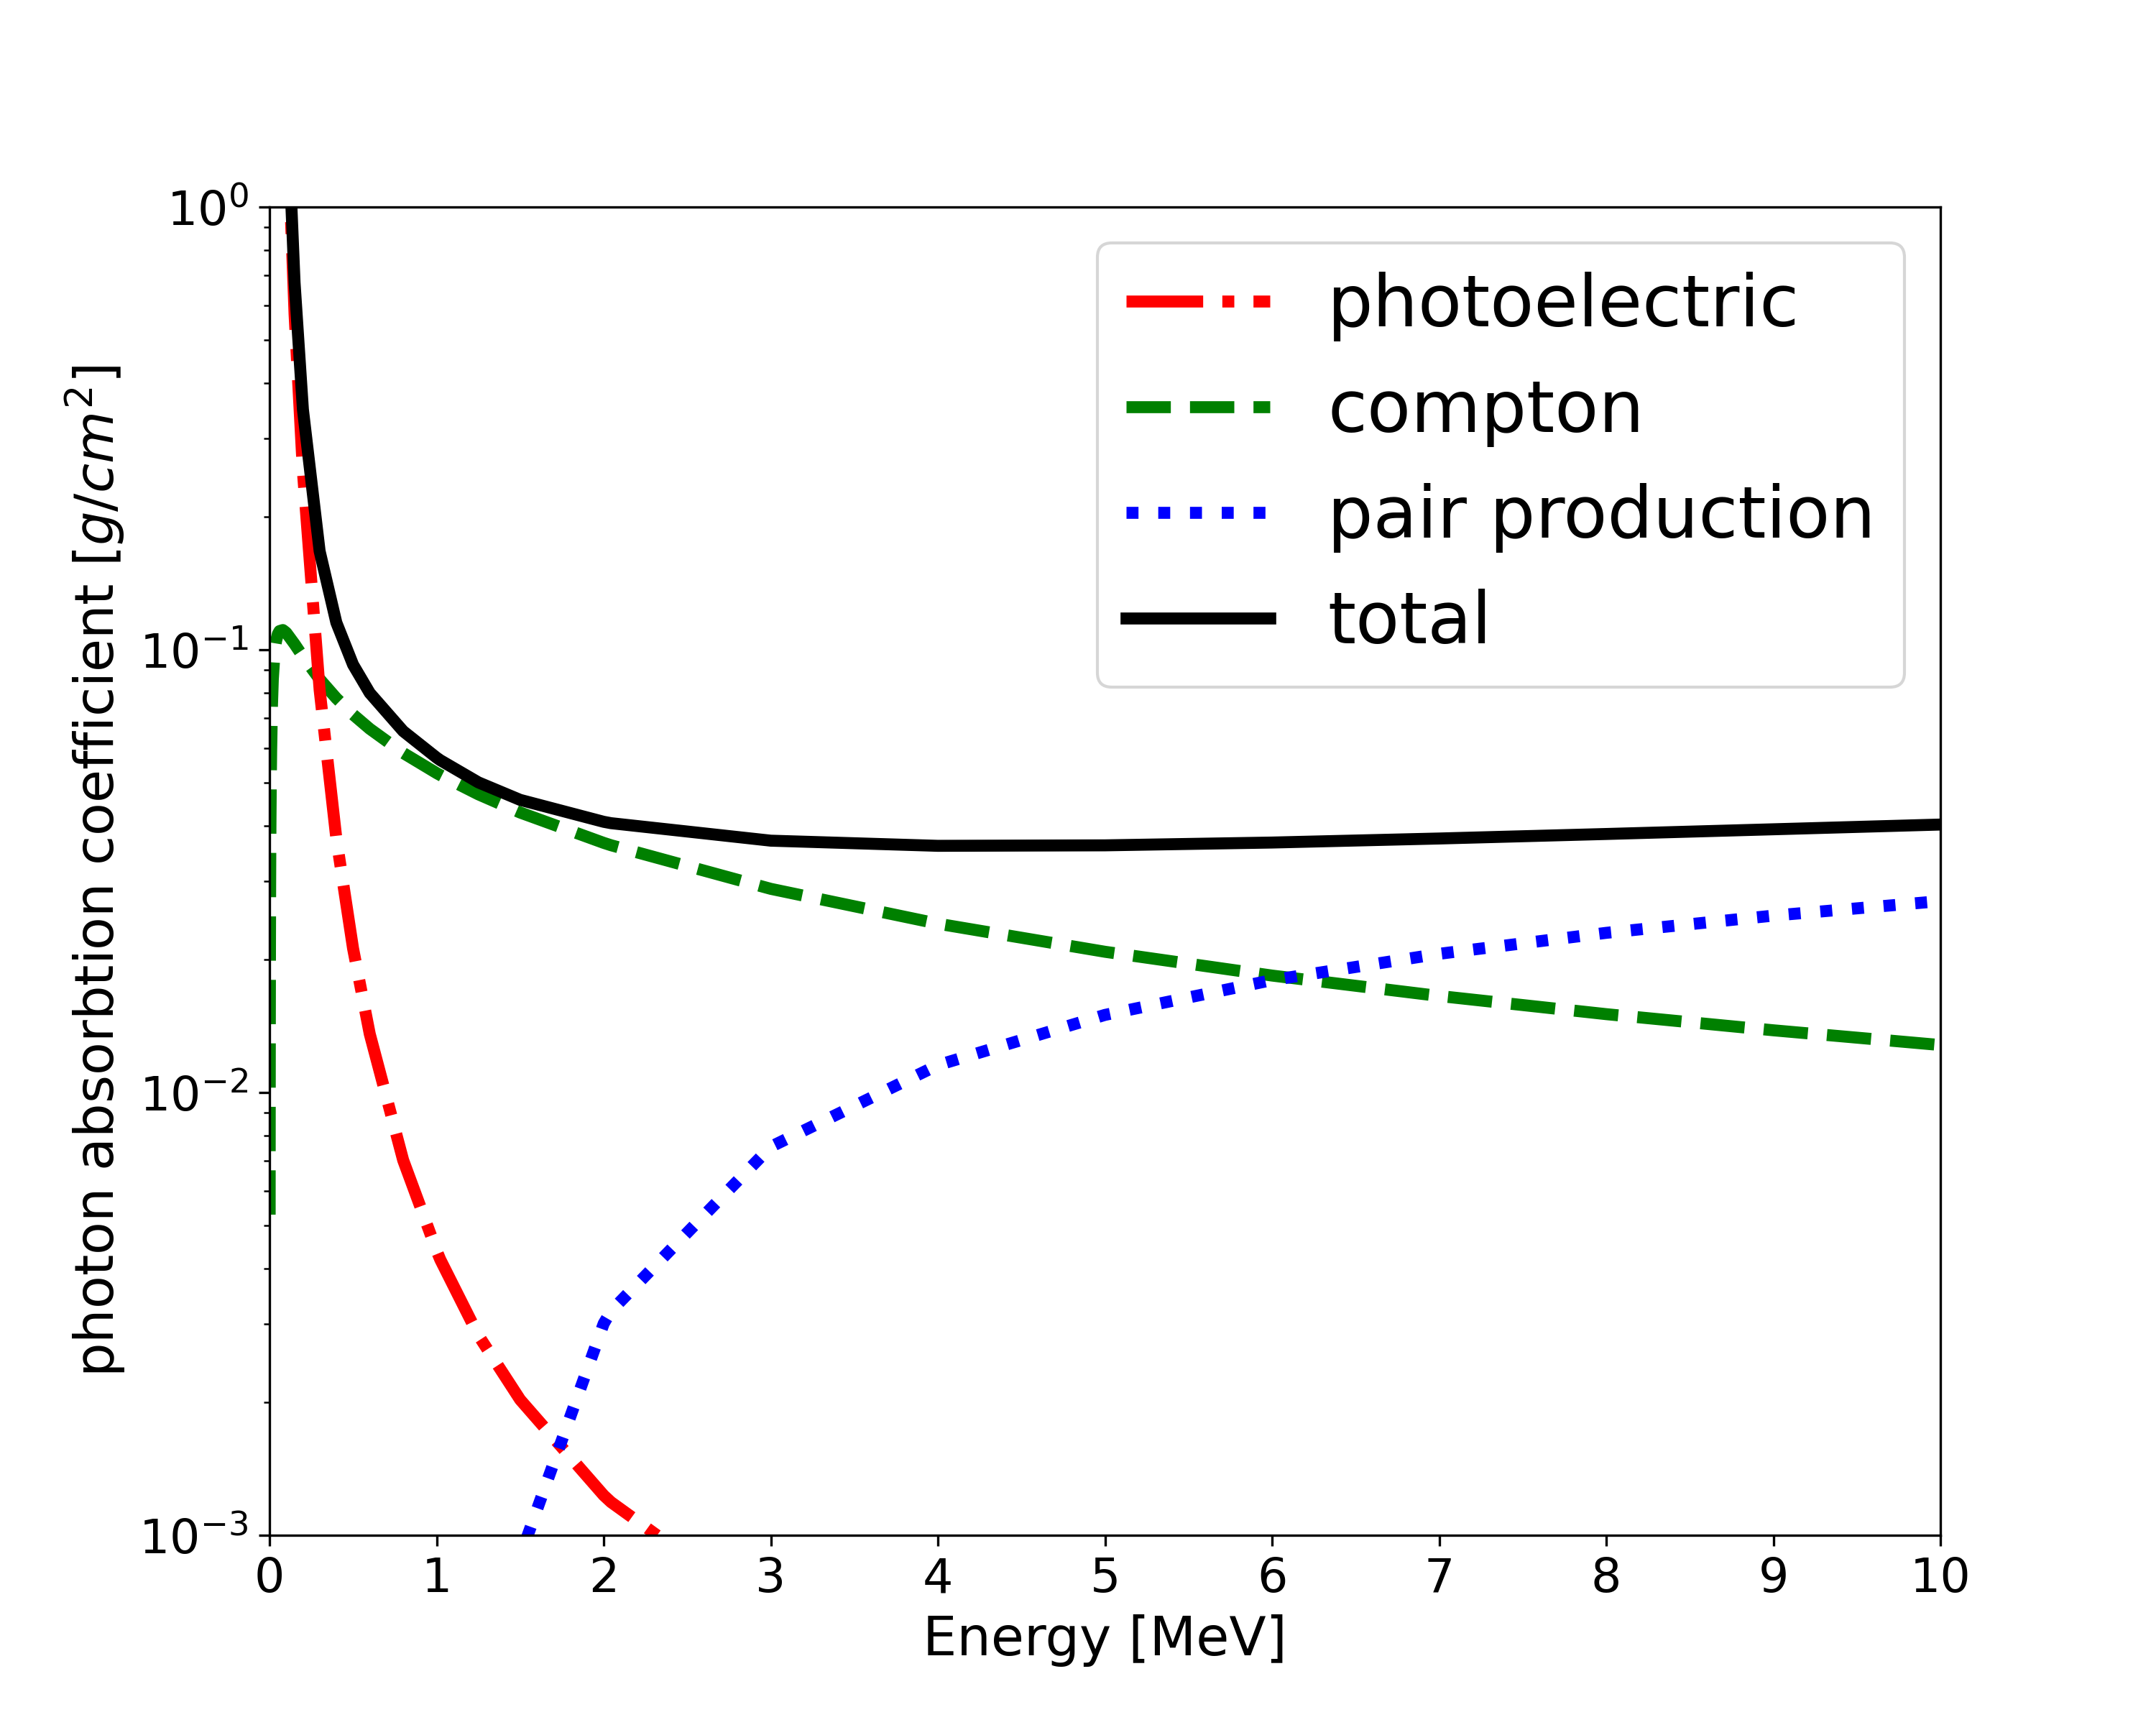
\includegraphics[width=0.95\textwidth]{Figures/csi_attuenuation.png}
        \caption{Mass attenuation coefficients for photons in CsI in the range from $100$ keV to $10$ MeV according to XCOM database \cite{seltzer2010xcom}.}
        \label{fig:csi}%
\end{figure}
At photon energies below approximately $300$ keV, the photoelectric effect dominates the interaction cross-section. As the photon energy increases, Compton scattering becomes the predominant process. For photon energies exceeding the pair production threshold ($E_{\gamma} > 2m_{e}c^2 \approx 1.022 MeV$), electron-positron pair creation becomes possible and is the dominant interaction mechanism above $E_{\gamma} \approx 6$ MeV.\newline
Compton scattering broadens the clustering by the deflection of the incident gamma ray. According to the Klein–Nishina formula, the scattering is predominantly forward-focused for moderate to high photon energies \cite{klein1929streuung}, leading to clusters in neighboring crystals.\newline
In the case of pair production, which occurs above the $2m_ec^2$ threshold, the resulting annihilation of the positron yields two $511$ keV gamma photons. These secondary photons often escape the initial interaction site, leading to a significant fraction of the incident photon’s energy being deposited in multiple detector elements.\newline
For gamma rays emitted by nuclei at rest, this behavior gives rise to well-defined single- and double-escape peaks in the recorded energy spectra -- corresponding to the escape of one or both $511\,\mathrm{keV}$ photons, respectively -- if these photons exit the cluster volume without interaction.\newline
In experiments involving relativistic ions, such as those conducted at $R^3B$, Doppler broadening significantly distorts spectral features, including single- and double-escape peaks\cite{knoll2010radiation}. This effect hinders accurate reconstruction of the photon energy and complicates the extraction of absolute gamma-ray yields and reaction cross sections.

\subsubsection{The Standard R3B Clustering Algorithm}
In the standard data acquisition (DAQ) configuration, all CALIFA detector hits occurring within a $\pm 4\,\mu\mathrm{s}$ time window are grouped into a single event. Each individual hit $i$ in CALIFA is represented by a data structure containing the following calibrated information, as already introduced in Section~\ref{sec:qfs_protons}:
\begin{itemize}
    \item Energy deposit $E_i$
    \item Polar angle $\theta_i$
    \item Azimuthal angle $\phi_i$
    \item Time stamp $t_i$ (via White Rabbit  Precision Time Protocol \cite{lipinski2011white})
\end{itemize}
In the standard R3B clustering approach, the time information $t_i$ is not utilized during the spatial reconstruction of clusters.\newline
The initial stage of the clustering algorithm begins by sorting all hits in descending order of energy. A user-defined geometric condition, typically a conical cluster shape with a default aperture of $0.25\,\mathrm{rad}$, is applied. This value has been found to provide an optimal compromise between compact high-energy clusters from light charged particles and more diffuse gamma-ray showers.\newline
The hit with the highest energy defines the seed or center of the first cluster. The algorithm then iterates through the remaining hits and includes each hit in the current cluster if it lies within the specified cone aperture relative to the seed direction. Once the list is fully processed for the current cluster, the next highest-energy unassigned hit becomes the seed of a new cluster. This procedure repeats until no unassigned hits remain.

\subsection{Data Simulation and Selection}

\subsubsection{Simulation Setup}
To evaluate and compare the clustering algorithms presented in this work, simulated datasets are employed to assess their performance. For both unsupervised approaches, such as agglomerative clustering, and supervised machine learning methods, such as the Edge Detection Neural Network, which will both be introduced in detail in the following section, access to ground truth labels is required. For this purpose, the R3BROOT framework~\cite{bertini2011r3broot} with a Geant4-based Monte Carlo \cite{agostinelli2003geant4} backend was employed.\newline
The CALIFA detector geometry used in the simulation corresponds to the configuration implemented in early 2024. At that time, the iPhos region (polar angles $19^\circ$ -- $43^\circ$) was fully instrumented, while only the forward half of the Barrel region ($43^\circ$ -- $87^\circ$) was active. The forward-most CEPA region ($7^\circ$ -- $19^\circ$) was not yet equipped.\newline
Gamma-ray energies were sampled from a uniform distribution between $0.3\,\mathrm{MeV}$ and $10\,\mathrm{MeV}$. The interaction of the primary gamma rays with the CsI(Tl) scintillation material was modeled using Geant4 transport physics.\newline
To emulate realistic event topologies, three gamma rays were generated per event, resulting in multiple detector hits. Timing information was coarsely simulated by assigning each primary gamma a random emission time within the $\pm 4\,\mu\mathrm{s}$ event window. The corresponding hit times were then Gaussian-smeared with a standard deviation of $200\,\mathrm{ns}$ to reflect typical electronic channel timing variations.\newline
The resulting dataset was split into training and test subsets, comprising 13{,}000 and 7{,}000 events, respectively.
\subsubsection{Performance Metrics}\label{s_sec:metrics}
To quantitatively assess the performance of the clustering algorithms presented in this work, a set of four custom metrics was defined. Three of these are event-based, while an optional fourth metric evaluates clustering quality on a per-cluster basis:
\begin{itemize}
    \item \textbf{True Positive (TP)}: All hits in an event are correctly assigned to their respective clusters.
    \item \textbf{False Positive (FP)}: At least one hit in an event is incorrectly merged into a cluster it does not belong to.
    \item \textbf{False Negative (FN)}: At least one hit is not merged into its true cluster and instead forms a spurious cluster.
    \item \textbf{False Mixed (FM)}: An event is classified as false mixed if it contains both FP and FN characteristics—i.e., at least one hit is incorrectly merged, and at least one true cluster is partially reconstructed.
\end{itemize}
In addition, a cluster-based metric is defined:
\begin{itemize}
    \item \textbf{Well Reconstructed (WR)}: The ratio of correctly reconstructed clusters to the total number of true clusters in the dataset.
\end{itemize}
These metrics allow a comprehensive evaluation of clustering accuracy, robustness, and failure modes.\newline
Special attention must be given to the false negative rate, which is closely associated with pair creation and subsequent annihilation processes. These processes produce widely spread hits that cannot be merged using the standard R3B clustering method, thereby motivating the development of a multi-layer perceptron architecture to improve clustering performance at the boundaries.\newline

\subsection{Agglomerative Clustering Model}
To incorporate temporal information into the clustering process---unlike the standard R3B algorithm, which omits it---a generic, well-established method was adopted: agglomerative clustering \cite{Nielsen2016} as implemented in the \texttt{SciPy} library \cite{virtanen2020scipy}. This unsupervised learning algorithm enables flat clustering based on hierarchical linkage with a user-defined threshold.\newline
Each hit was mapped into spherical coordinates \((\theta, \phi, r)\), where the radial component \(r\) encodes time information. To ensure non-negative radii, the acquisition time window of \(\pm 4\,\mu\mathrm{s}\) was shifted by \(+4.5\,\mu\mathrm{s}\). The Ward linkage criterion \cite{nielsen2016hierarchical}, which minimizes intra-cluster variance, was employed as the distance metric.\newline
The threshold parameter was optimized to yield the best performance according to the custom-defined \textit{true positive} (TP) and \textit{well reconstructed} (WR) metrics. A comparison between the standard R3B clustering and the agglomerative method is presented in Figure~\ref{fig:r3b_agglo_metrics}.
\begin{figure}[!htb]
       \centering
       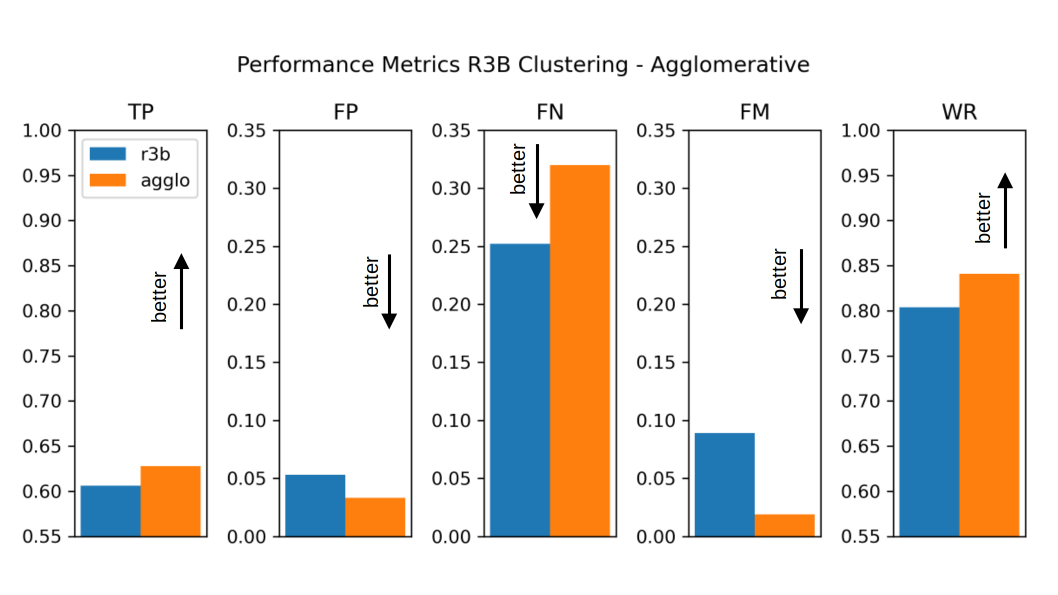
\includegraphics[width=0.95\textwidth]{Figures/r3b_agglo_arrows.png}
       \caption{Comparison of clustering performance on the test dataset using standard R3B clustering (blue) and agglomerative clustering (orange) incorporating hit-time information. The dataset comprises simulated $\gamma$-rays with energies uniformly distributed between 0.3 and 10\,MeV. The metrics shown include event-based and cluster-based measures: \textit{TP}, \textit{FP}, \textit{FN}, \textit{FM}, and \textit{WR}; see also Subsection~\ref{s_sec:metrics}.}
       \label{fig:r3b_agglo_metrics}%
\end{figure}
As shown in Figure~\ref{fig:r3b_agglo_metrics}, the agglomerative clustering algorithm demonstrates improved performance both on an event level (true positive rate) and on a cluster level (correctly reconstructed clusters). However, this improvement is accompanied by an increased false negative rate, indicating that the algorithm tends to under-merge hits near the edges of clusters. This limitation motivated the development and application of an edge detection neural network, which is introduced in the following subsection.

\subsection{Edge Detection Neural Network}
To enhance the clustering performance, particularly at the boundaries of hit distributions, a multi-layer perceptron architecture was developed using the Pytorch library~\cite{imambi2021pytorch} to perform pairwise classification of detector hits. This model is applied either to individual raw hits or to hits pre-clustered via agglomerative clustering, on an event-by-event basis.

The model takes 12 input features for each hit pair $(i, j)$: absolute values of energy $(E_i, E_j)$, polar angle $(\theta_i, \theta_j)$, azimuthal angle $(\phi_i, \phi_j)$, and time $(t_i, t_j)$. Additionally, four differential features are computed: $\Delta E = |E_i - E_j|$, $\Delta \theta = |\theta_i - \theta_j|$, $\Delta \phi = |\phi_i - \phi_j|$, and $\Delta t = |t_i - t_j|$. These differential inputs are helpful for training stability and convergence with our limited model sizes tested. In particular, $\Delta \phi$ resolves the discontinuities caused by the periodicity of the azimuthal angle (e.g., distinguishing between $\phi = 355^\circ$ and $\phi = 5^\circ$), which would otherwise introduce large erroneous differences in angular comparisons.

Of the 12 features, only the hit time is normalized to the $[0, 1]$ interval; all other values are used in their native physical units.
The neural network architecture takes the 12-dimensional input vector and passes it through a fully connected feed-forward network with one hidden layer of $10^3$ nodes, followed by a ReLU activation. Two additional hidden layers, each with $10^2$ nodes, are applied sequentially. The output layer consists of a single node with a sigmoid activation, yielding a score in the interval $[0, 1]$, where values close to 1 indicate that the hits (or clusters) are likely to originate from the same event cluster.\newline

Training is performed using the binary cross-entropy loss function \cite{mannor2005cross,de2005tutorial} and stochastic gradient descent (SGD) \cite{newton2018recent} with a fixed learning rate of $5 \times 10^{-3}$. Given the moderate size of the training dataset, full-batch training is employed without mini-batching. The model is trained for $8 \times 10^4$ epochs. After training, a threshold is applied to the prediction scores to classify hit pairs. This threshold is tuned to optimize the performance across all defined metrics, as described in Subsection~\ref{s_sec:metrics}. Final clusters are then formed by grouping all connected hit pairs based on the predicted associations.

The edge detection NN was implemented and tested in three configurations:
\begin{itemize}
    \item \textbf{Plain Edge NN:} The model is applied directly to individual hits without any pre-clustering. All clustering is performed based solely on the NN predictions.
    \item \textbf{R3B + Edge NN:} The data are first clustered using the standard R3B clustering algorithm as an initial clean-up step. For each resulting cluster, an energy-weighted center of mass is calculated, replacing individual hits. The  NN is then trained exclusively on false negative cases, i.e., events where reconstructed clusters exhibit detached hits. In application, the R3B standard clustering is first applied to the test data, followed by the NN to refine cluster boundaries and reduce the false negative rate as clean-up step.
    \item \textbf{Agglo + Edge NN:} This strategy mirrors the R3B+Edge approach, with the key difference that time information is incorporated. As in the R3B+Edge model, the NN is trained on false negative cases to perform a final clean-up step after pre-clustering the hits using the agglomerative clustering algorithm described in the previous subsection. The significant reduction of the false negative rate achieved by the clean-up step in the Agglo+Edge implementation is demonstrated in Figure~\ref{fig:2_1_mev_r3b_aggloNN}, which compares the reconstructed energy spectra from simulations of monoenergetic 2.1~MeV gamma events using the R3B standard clustering and the Agglo+Edge method.
\end{itemize}
\begin{figure}[!htb]
        \centering
        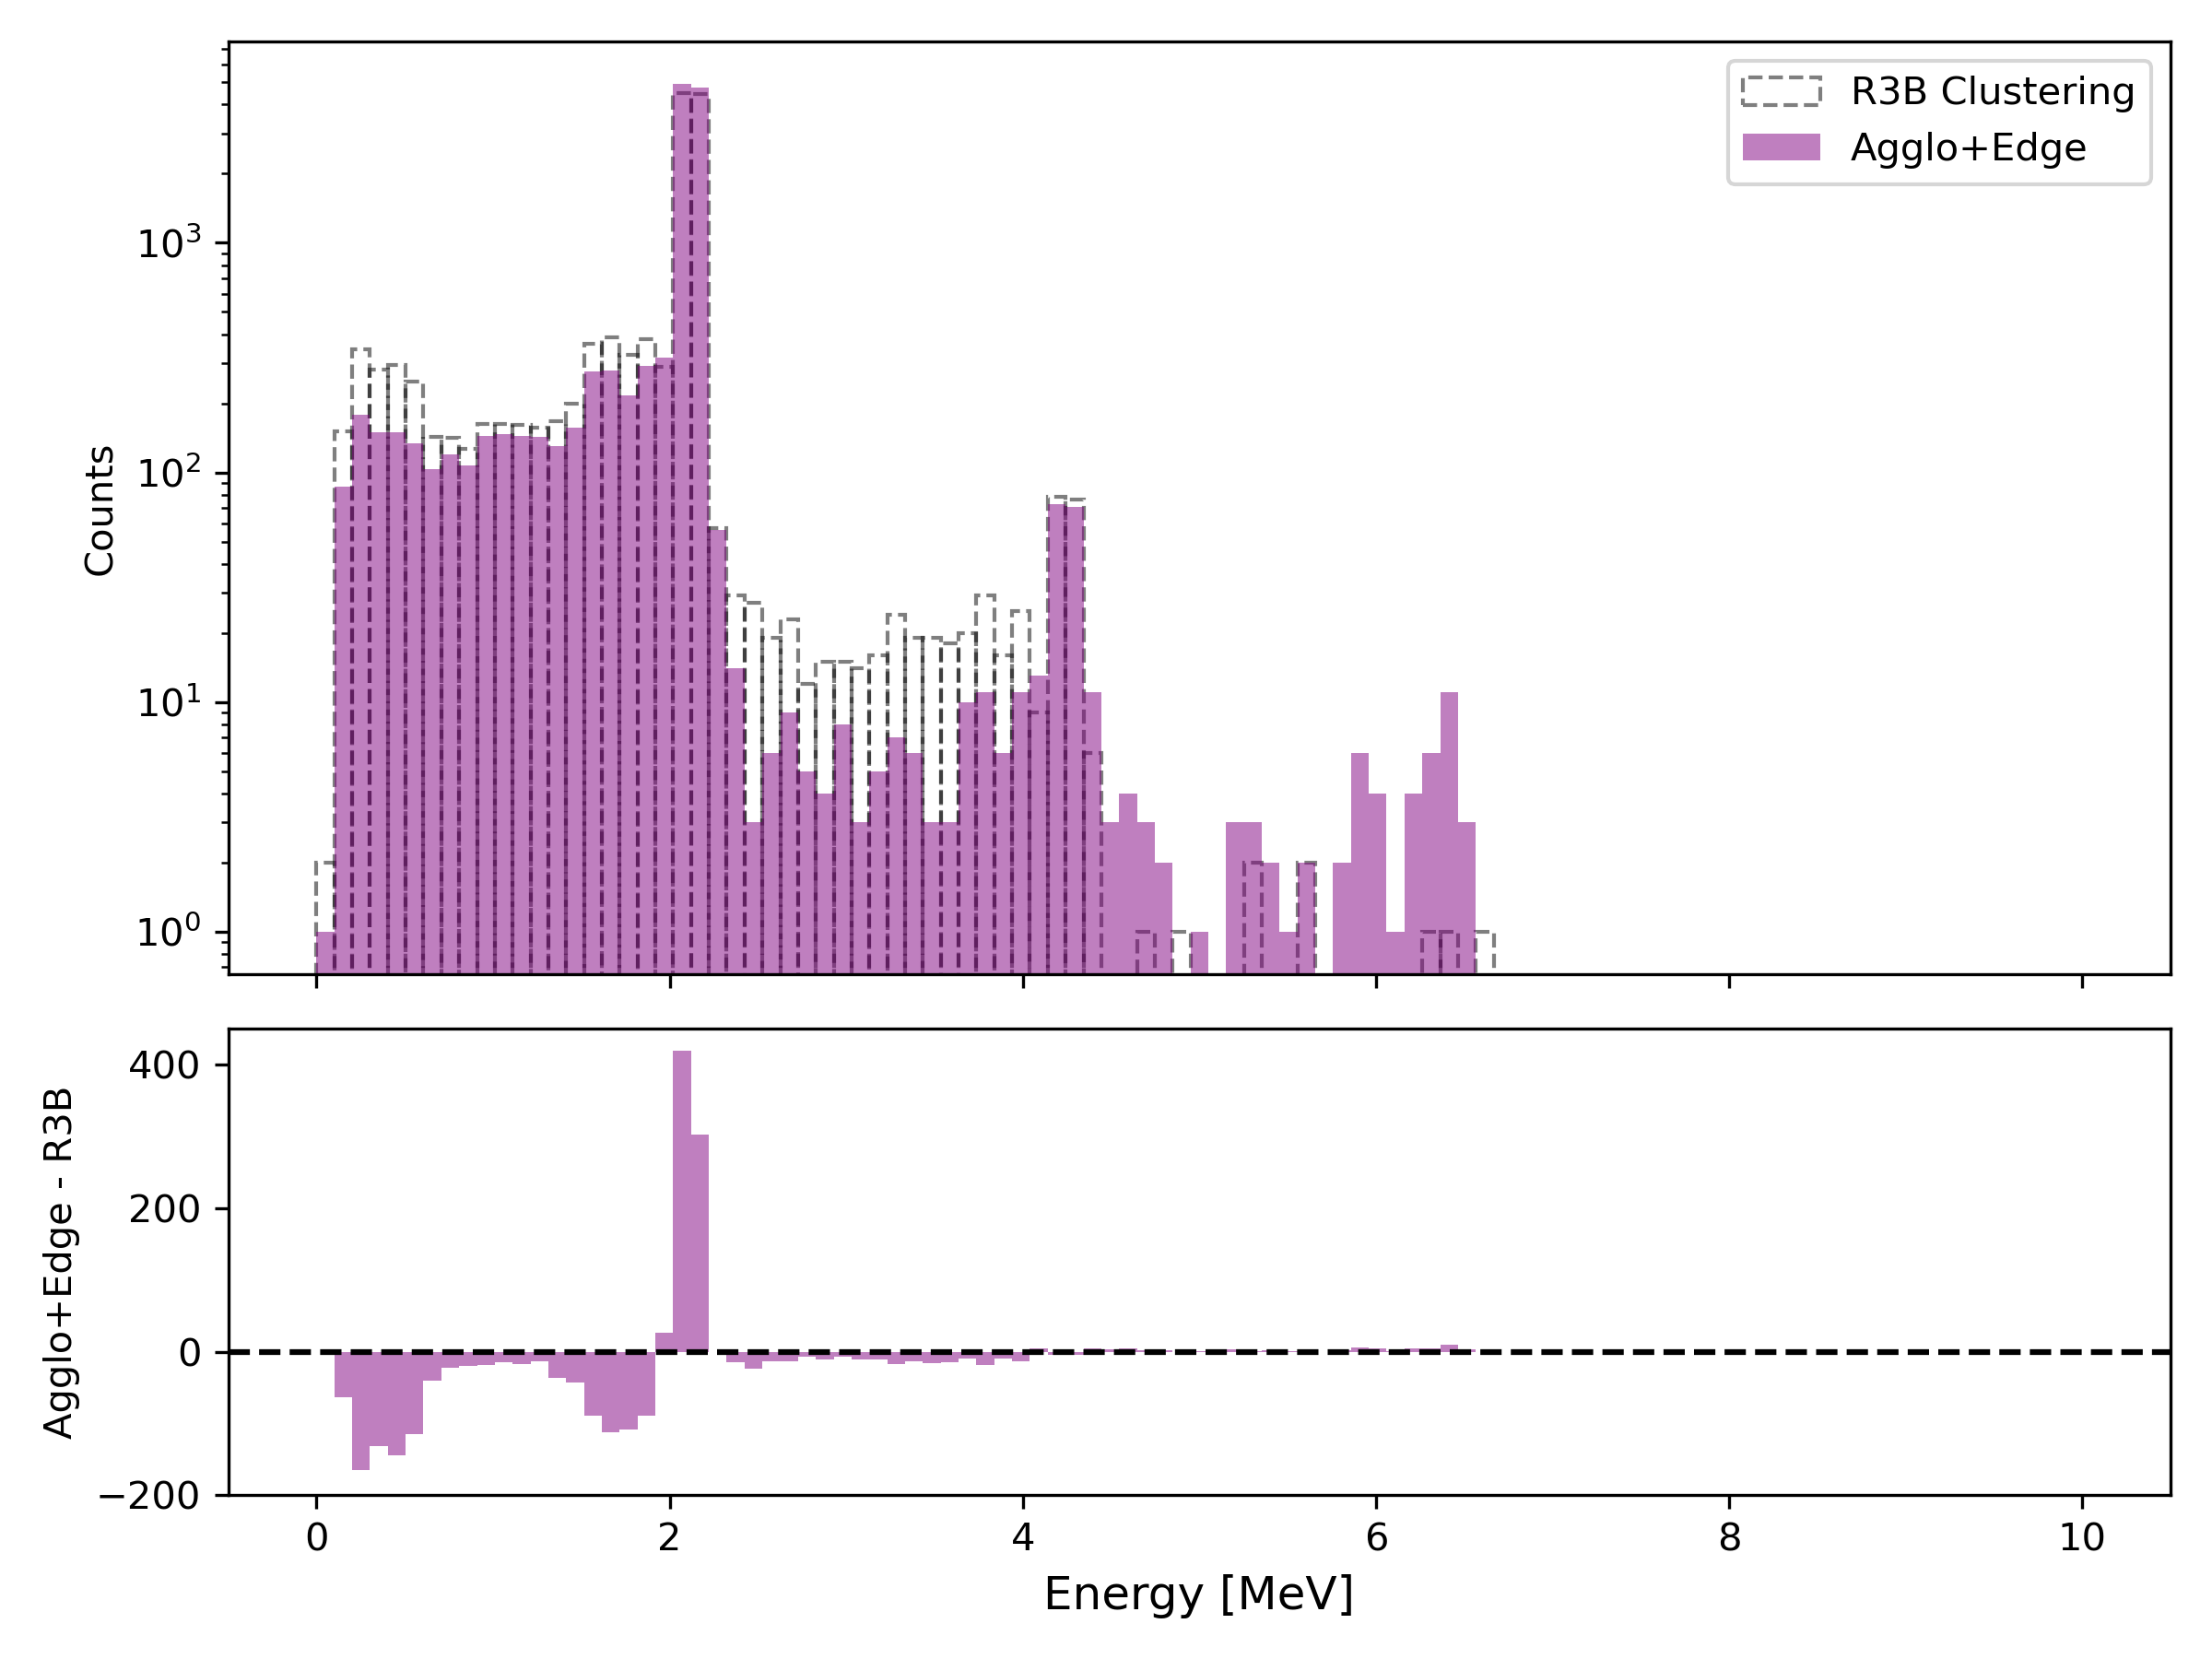
\includegraphics[width=0.95\textwidth]{Figures/spec_2_1agglo_edge_vsr3b.png}
        \caption{Reconstructed gamma energy spectrum from simulated events, each consisting of three 2.1~MeV gamma photons. The upper panel shows the comparison between the standard R3B clustering and the Agglo+Edge method. The lower panel displays the bin-by-bin count difference between the two approaches. The Agglo+Edge model demonstrates a significant improvement by successfully reattaching escaped hits, notably in cases where sparse energy deposits around 1.6~MeV and 0.5~MeV result from pair production and subsequent annihilation processes of the original gamma photons. This clean-up step leads to a marked reduction in false negatives compared to the standard R3B clustering.}
        \label{fig:2_1_mev_r3b_aggloNN}%
\end{figure}

\subsection{Results}
\begin{table}[h!]
\begin{center}
\resizebox{0.95\textwidth}{!}{%
\begin{tabular}{||c| c| c |c | c|| c|}
 \hline
 Clustering Model & TP($\uparrow$) & FP($\downarrow$) & FN($\downarrow$) & FM($\downarrow$) & WR($\uparrow$) \\ [0.5ex]
 \hline\hline
 R3B Standard Clustering & 60.6 & 5.3 & 25.2 & 8.9 & 80.4 \\
 \hline
 Agglomerative Clustering & 62.8 & \textbf{3.3} & 32.0 & 1.9 & 84.1 \\
 \hline
 Edge Clustering (no time) & 63.4$\pm$0.3 & 7.2$\pm$0.3 & 24.8$\pm$0.7 & 4.6$\pm$0.1 & 82.4$\pm$0.1 \\
 \hline
 Edge Clustering (with time) & 74.7$\pm$0.5 & 3.4$\pm$0.6 & 20.5$\pm$1.3 & 1.4$\pm$0.1 & 89.2$\pm$0.1 \\
 \hline
 R3B + Edge (no time) & 67.4$\pm$0.3 & 8.5$\pm$0.3 & 16.0$\pm$0.4 & 8.0$\pm$0.3 & 82.2$\pm$0.1 \\
 \hline
 Agglo + Edge (with time) & \textbf{81.3$\pm$0.3} & 5.1$\pm$0.0 & \textbf{12.2$\pm$0.3} & \textbf{1.5$\pm$0.1} & \textbf{91.0$\pm$0.1} \\
 \hline
\end{tabular}
}
\end{center}
\caption{Summary of performance metrics as defined in Subsection~\ref{s_sec:metrics}, evaluated for the different clustering algorithms. The models \textit{R3B Standard Clustering}, \textit{Edge Clustering (no time)}, and \textit{R3B + Edge (no time)} utilize only angular and energy information on a per-hit basis for cluster reconstruction. In contrast, \textit{Agglomerative Clustering}, \textit{Edge Clustering (with time)}, and \textit{Agglo + Edge (with time)} additionally incorporate time-of-hit information into the clustering process. Uncertainties reported for the four edge detection neural network variants correspond to the standard deviation of the results obtained from ten independent training runs.}
\label{tab:results}
\end{table}
The results of this study are summarized in Table~\ref{tab:results}, organized according to increasing levels of reconstruction complexity. For completeness, the previously obtained results from the comparison between the "baseline" R3B standard clustering algorithm and the agglomerative model are also included.\newline
The agglomerative model shows improved performance over the R3B baseline in terms of both event-level true positives (TP) and cluster-level (WR) values. However, it exhibits inferior performance with respect to the false negative (FN) rate, indicating a tendency to miss relevant hits during reconstruction. This limitation motivated the development of an Edge Detection Neural Network, initially evaluated as a standalone clustering algorithm and subsequently integrated into the agglomerative framework, yielding the combined model denoted as \textit{Agglo + Edge}.\newline
The \textit{Agglo + Edge} model demonstrates superior performance across all evaluated metrics, achieving an overall correct reconstruction rate of 81.3\%, significantly outperforming the \textit{R3B Standard Clustering} algorithm, which reaches 60.6\%.\newline
A visual representation of an event, contrasting the incorrectly merged hits from the R3B standard clustering with the correctly reconstructed clustering using the Agglo+Edge model, is shown in Figure~\ref{fig:comparison_r3b_agglo_edge}.\newline
\begin{figure}[htbp]
    \centering
    \begin{subfigure}[b]{0.45\textwidth}
        %\includegraphics[width=\textwidth]{best_example_bad_r3b.png}
        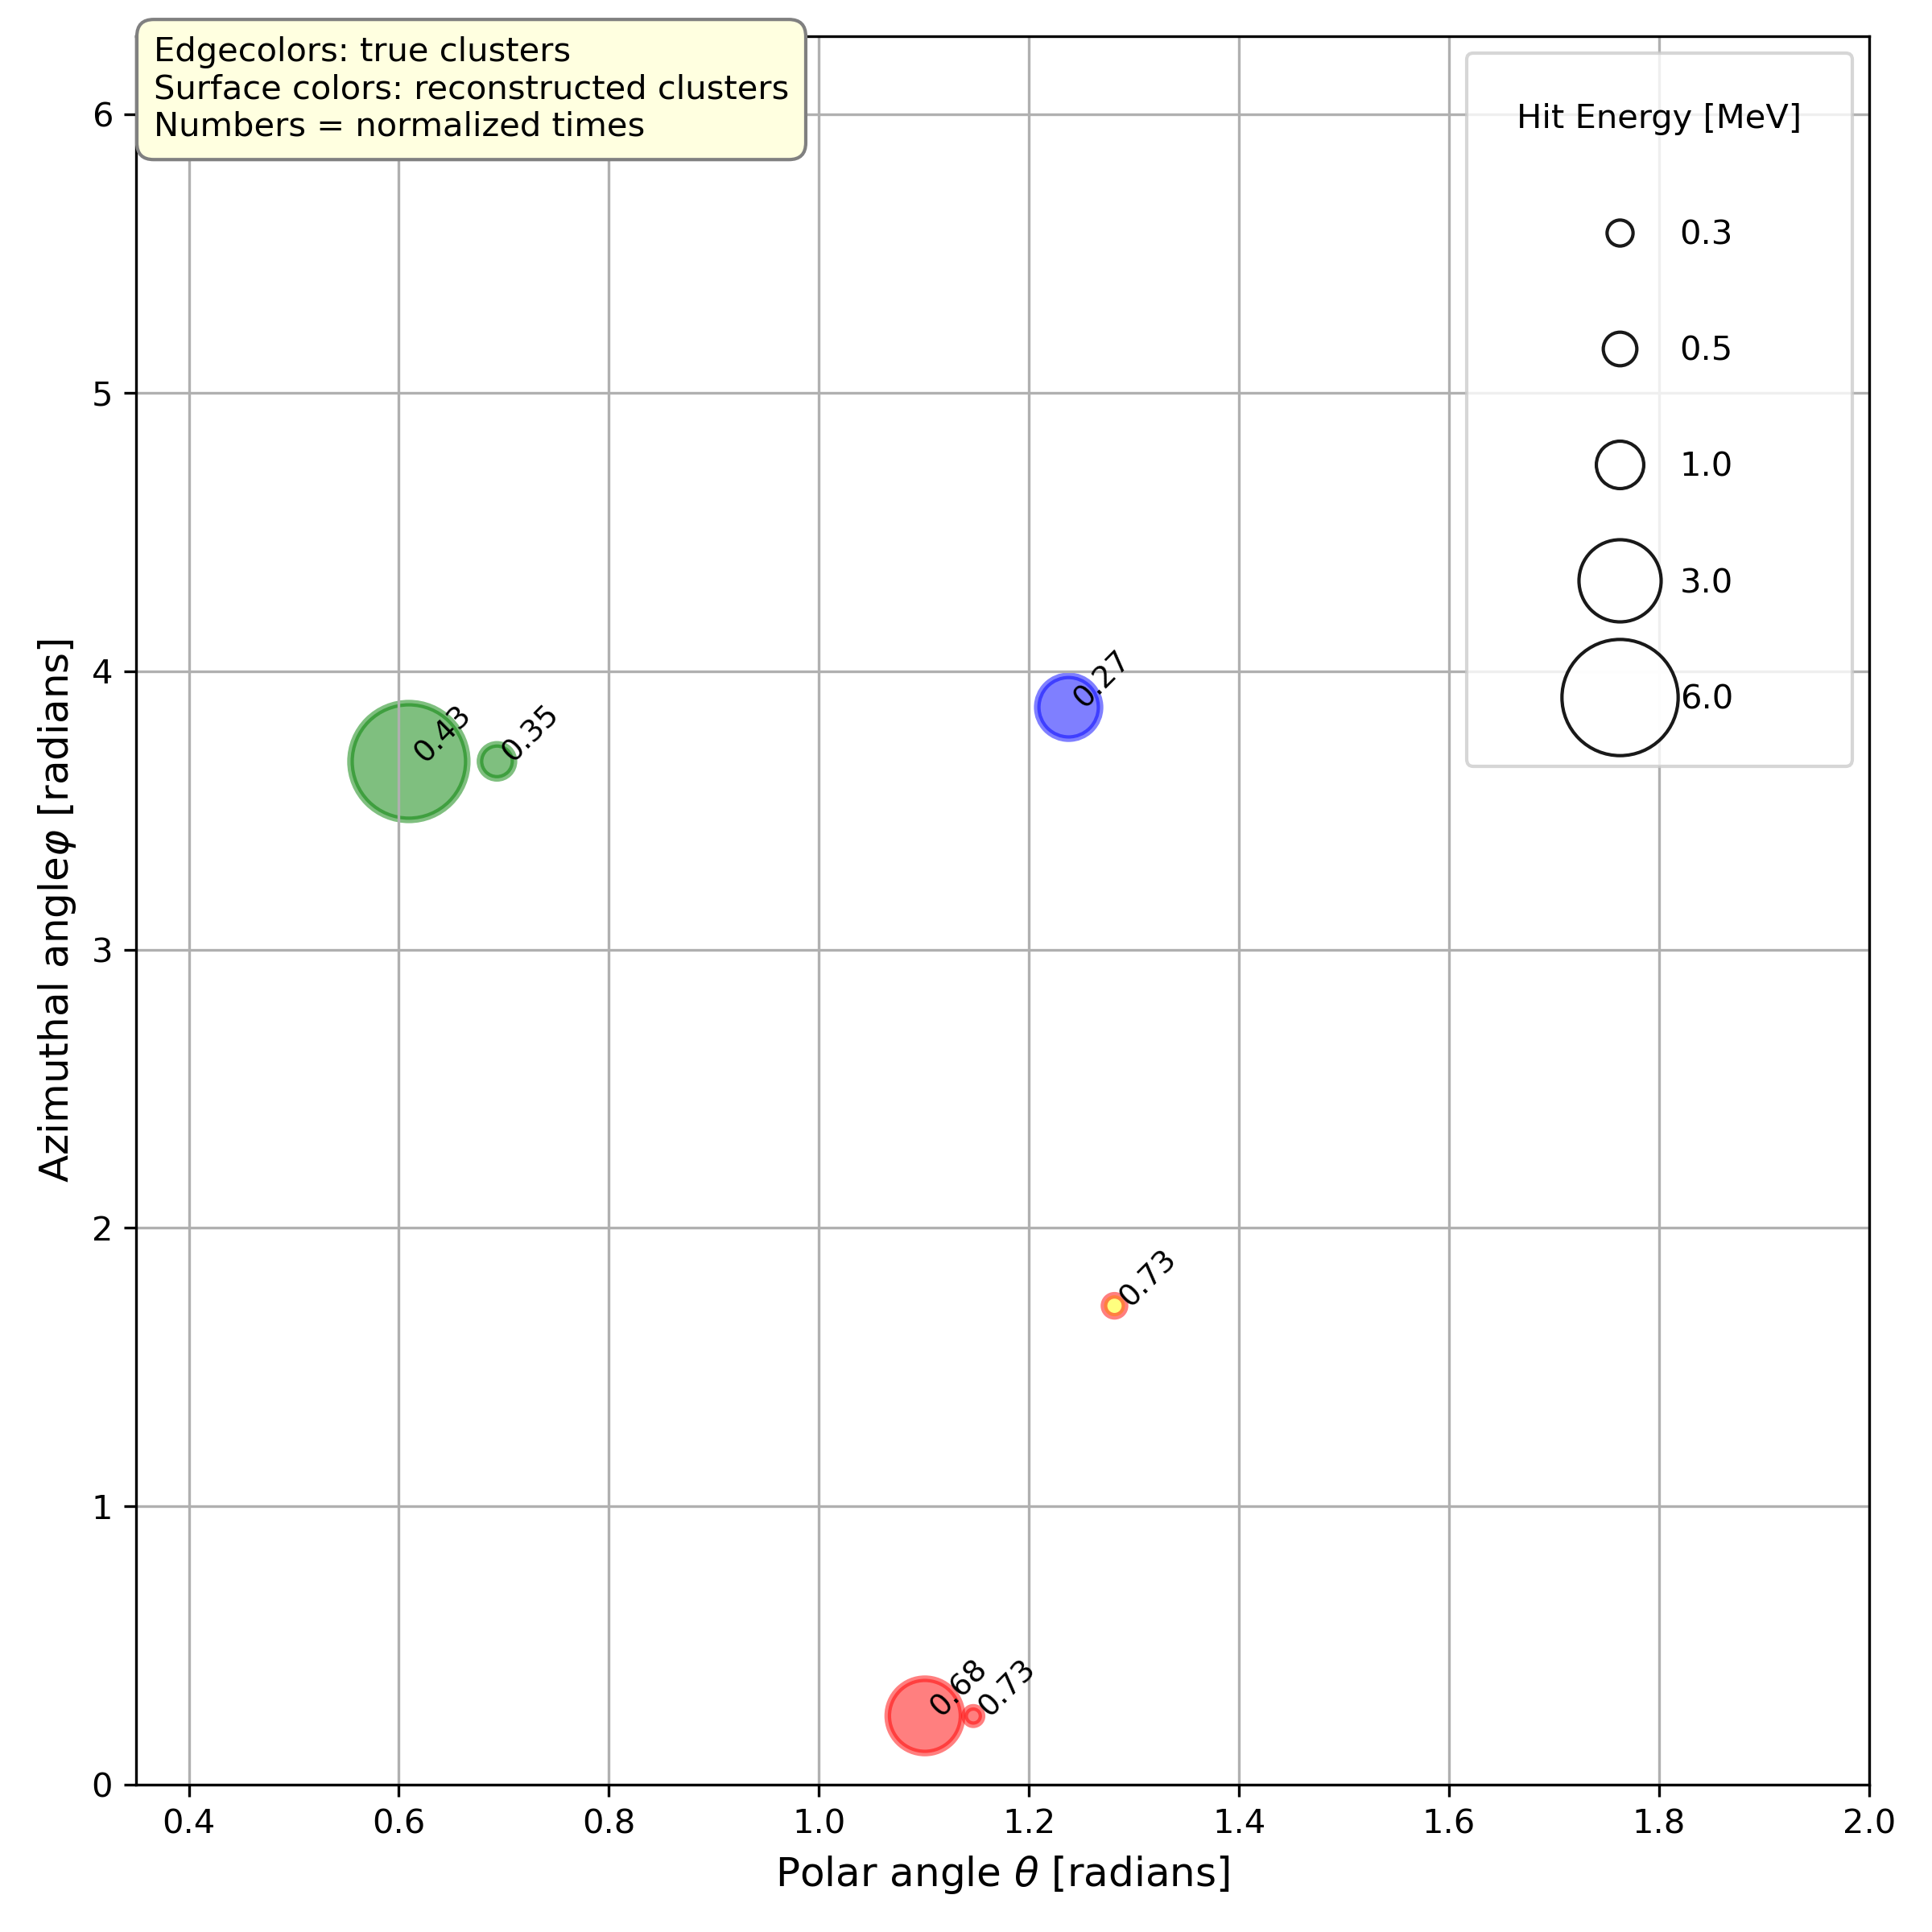
\includegraphics[width=\textwidth]{Figures/bad_reco_paper.png}
        \centering
        \subcaption{R3B standard clustering: the red-edged cluster with sparse hits is incorrectly split up into two clusters.}
        \label{fig:subfig1}
    \end{subfigure}
    \hfill
    \begin{subfigure}[b]{0.45\textwidth}
        %\includegraphics[width=\textwidth]{best_example_good_agglo_edge.png}
        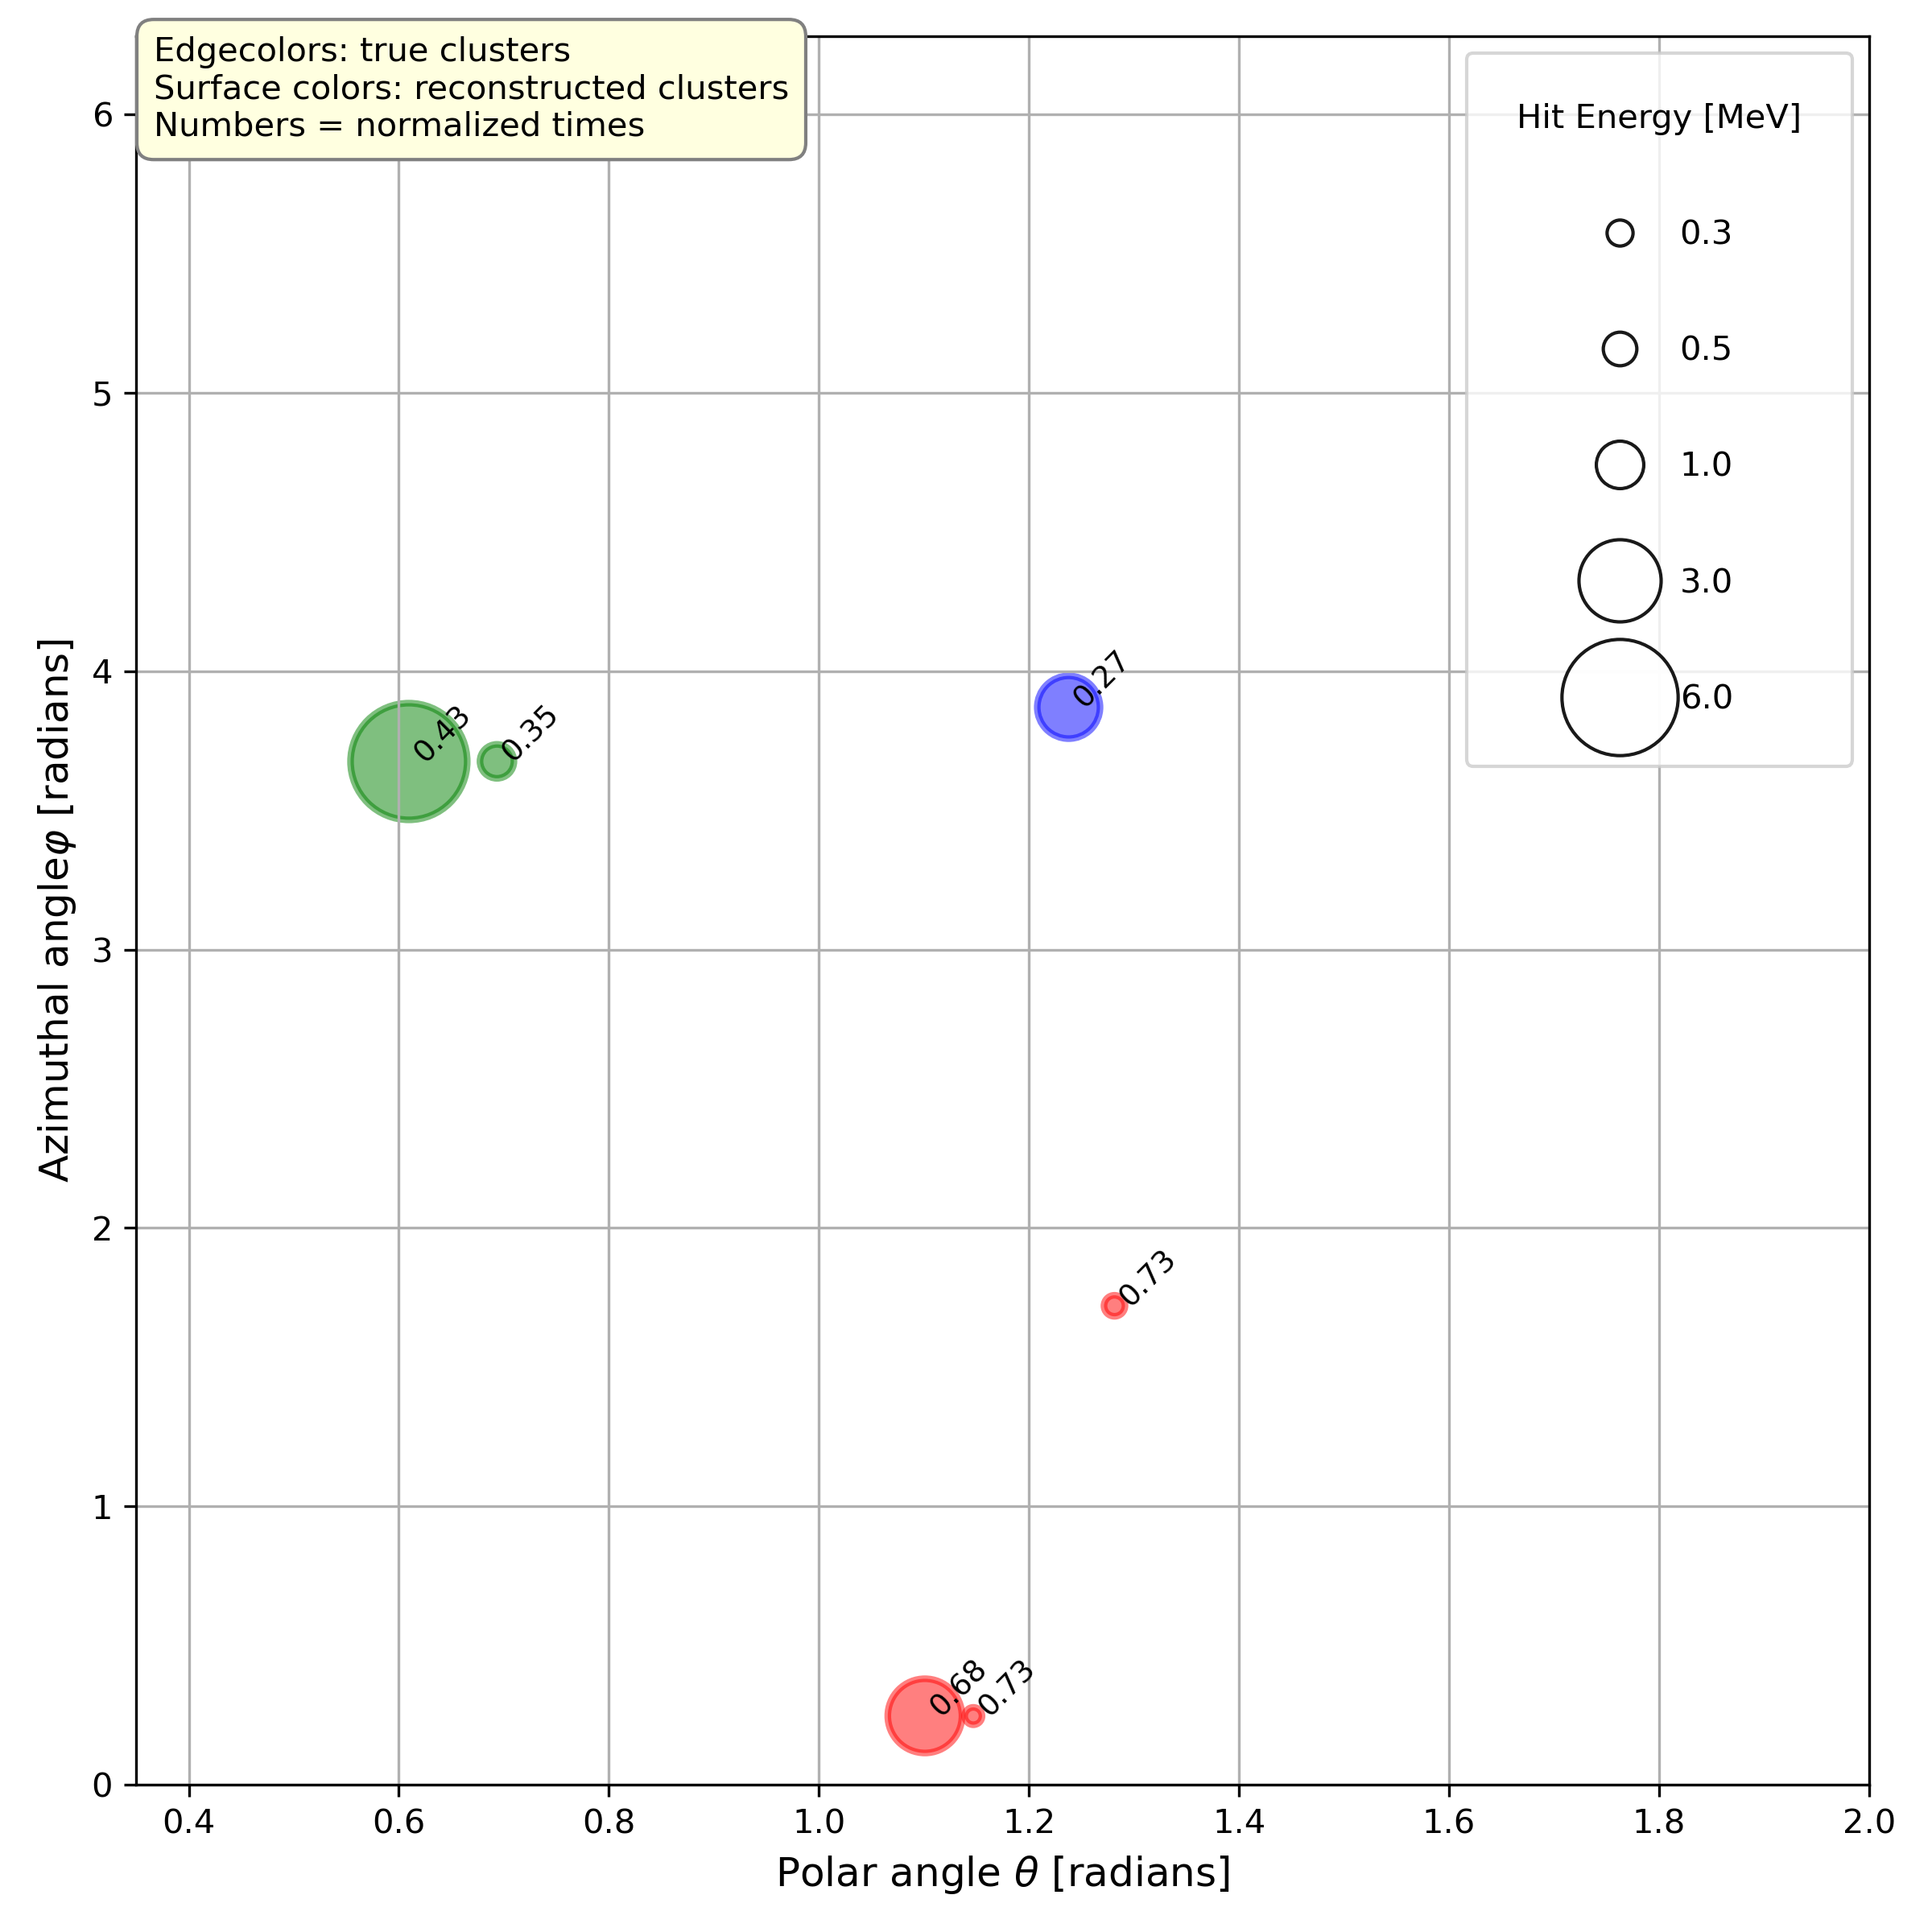
\includegraphics[width=\textwidth]{Figures/good_reco_paper.png}
        \centering
        \subcaption{Agglo+Edge clustering: successful reattaching of sparse hits.}
        \label{fig:subfig2}
    \end{subfigure}
    \caption{Exemplary event with three simulated gamma photons in the energy range of 0.3–10~MeV, comparing the reconstruction performance of the R3B standard clustering and the Agglo+Edge method.}
    \label{fig:comparison_r3b_agglo_edge}
\end{figure}
To further explore the capabilities of neural network-based clustering approaches, two additional models were evaluated: a standalone \textit{Edge Detection Neural Network} and a hybrid approach combining \textit{R3B Standard Clustering} with edge-based postprocessing (\textit{R3B + Edge}). Notably, both of these models operate without incorporating time-of-hit information, similar to the R3B baseline. Nonetheless, both outperform the \textit{R3B Standard Clustering}, underscoring the potential of edge-based neural network models for improving cluster reconstruction in high-granularity detector systems.\newline
The edge detection NNs presented here represent a special case of Graph Neural Networks (GNNs)~\cite{battaglia2018relational}, which, along with the more sophisticated transformer models~\cite{vaswani2017attention,amatriain2023transformer}, have seen widespread adoption in particle physics over the past five years~\cite{dezoort2021charged,ju2021performance,van2024transformers}. Interestingly, for this application, using an unsupervised learning algorithm (agglomerative clustering) to first define a graph structure presented a powerful inductive bias for our application which much improved our results over the standalone edge-NN. One limitation of this approach is is cannot improve an overly aggressive pre-clustering (e.g, a false positive rate can never be decreased  in the clean-up step by the edge-NN). However, the necessity of reattaching edge hits to address the high false negative rate—exceeding the false positive rate by a factor of five in the baseline reconstruction (see Table~\ref{tab:results})—motivated this strategy.\newline
Subsequent work could consider also adding a subsequent cluster splitting step in an end-to-end optimizable algorithm.\newline
Although, in principle, transformers could learn the graph structure directly from hit distributions, initial tests showed limited performance, highlighting an opportunity for the community to further develop combined machine learning-based reconstruction methods.\newline


\subsection{Discussion and Outlook}
\begin{itemize}
\item maybe add the discussion from the paper-draft
\item add the note that it should maybe tried out to use much less nodes, factor 10-100
\item mention that these results are in the way to be published in NIM-A
\end{itemize}

